\section{Eingangsspannung bereinigen}
\label{Eingangsspannung bereinigen}

%% Describes our Opamps and Voltage divider
%% also reasoning for choosing those specific
%% values of resistor, power supply, etc.
Der GPIO Pin aus \ref{Mikrocontroller}, an dem die Spannung mithilfe eines Mikrocontrollers gemessen wird,
kann nur Spannung im Bereich $[0, 3.3]V$ messen.
Das Oszilloskop soll allerdings einen größeren Spannungsbereich $[-5, 5]V$ messen können.
Daher wird nun die Eingangsspannung bereinigt, sodass sie den Anforderungen des GPIO Pin genügt.

\subsection{Unbelastete Eingangsspannung}
\label{Unbelastete Eingangsspannung}
Der Stromkreis, der gemessen wird, soll nicht belastet werden, daher wird ein Opamp mit
hoher Eingangsimpedanz und einem Verstärkungsfaktor von $1$ benutzt.
Dies wird durch eine Rückkopplung des Ausgangs an den invertierten Eingang des Opamps erreicht.
\begin{figure}[h]
	\centering
	\includegraphics[width=0.7\textwidth]{images/schematic\_teil1\_unbelastet\_opamp.png}
	\caption{Schaltplan um den Eingangsstrom nicht zu belasten, Ausschnitt aus \ref{Gesamte_Schematic}}
\end{figure}


\subsection{Addition einer Offset-Spannung}
\label{Addition einer Offset-Spannung}

Nun gilt es den Spannungsbereich von $[-5, 5]V$ auf $[0, 10]V$ zu legen.
Dafür wird eine Offset-Spannung $U_{offset}$, die aus einem $V_{CC}$ Pin
des Mikrocontrollers stammt und mithilfe des Stepup Spannungsreglers auf $5V$ gebracht wird, zur Eingangsspannung dazu addiert.
Dies geschieht mit einem Nichtinvertierenden Summierverstärker, also ein Opamp der extern mit
Spannungsteilern, gemäß \autoref{fig:Opamp_Adder}, beschalten ist.
Der Opamp arbeitet also mit Spannungen im Bereich $[-5,10]V$,
daher muss der Bereich der Versorgungsspannung mindestens diese Spannungswerte enthalten.
Experimentell hat sich herausgestellt, dass der \textit{TS912IN} funktioniert, solange die Eingangsspannung
unterhalb von $1.7V$ der Versorgungsspannung liegt.
Daher wird für den Opamp großzügig eine positive Versorgungsspannung von $V^+_{CC} = 15V$ und eine 
negative von $V^-_{CC} = -15V$ gewählt.
Für die maximale Eingangsspannung gilt $\max(U_{in}) + U_{offset} = 5V + 5V = 10V < (15V - 1.7V)$
und für die minimale gilt $\min(U_{in}) + U_{offset} = -5V + 5V = 0V$.
Der Opamp funktioniert also für die definierte Eingangs- und Offsetspannung. \newline
Es gilt, laut \cite{Opamp_adder}, für die Ausgangsspannung $U_3$ des Opamps:
\begin{align*}
U_3 &= (U_{in} \cdot \frac{R_2}{R_1 + R_2} + U_{offset} \cdot \frac{R_1}{R_1 + R_2}) \cdot(1 + \frac{R_4}{R_3}) \\
	&= (U_{in} \cdot \frac{1}{2} + U_{offset} \cdot \frac{1}{2}) \cdot 2 \\
	&= U_{in} + U_{offset}
\end{align*}

\begin{figure}[h!]
	\centering
	\includegraphics[width=0.7\textwidth]{images/schematic\_teil2\_adder.png}
	\caption{Addition von $U_{in}$ und $U_{offset}$, Ausschnitt aus \ref{Gesamte_Schematic}}
	\label{fig:Opamp_Adder}
\end{figure}

%Eine Messung der Spannung von $U_{in}$ und $U_3$ mittels eines kommerziellen Oszilloskops zeigt,
%für eine Wechselspannung mit Amplitude $5V$, erfolgreich $U_3 = U_{in} + U_{offset}$:
%\begin{figure}[h!]
%	\centering
%	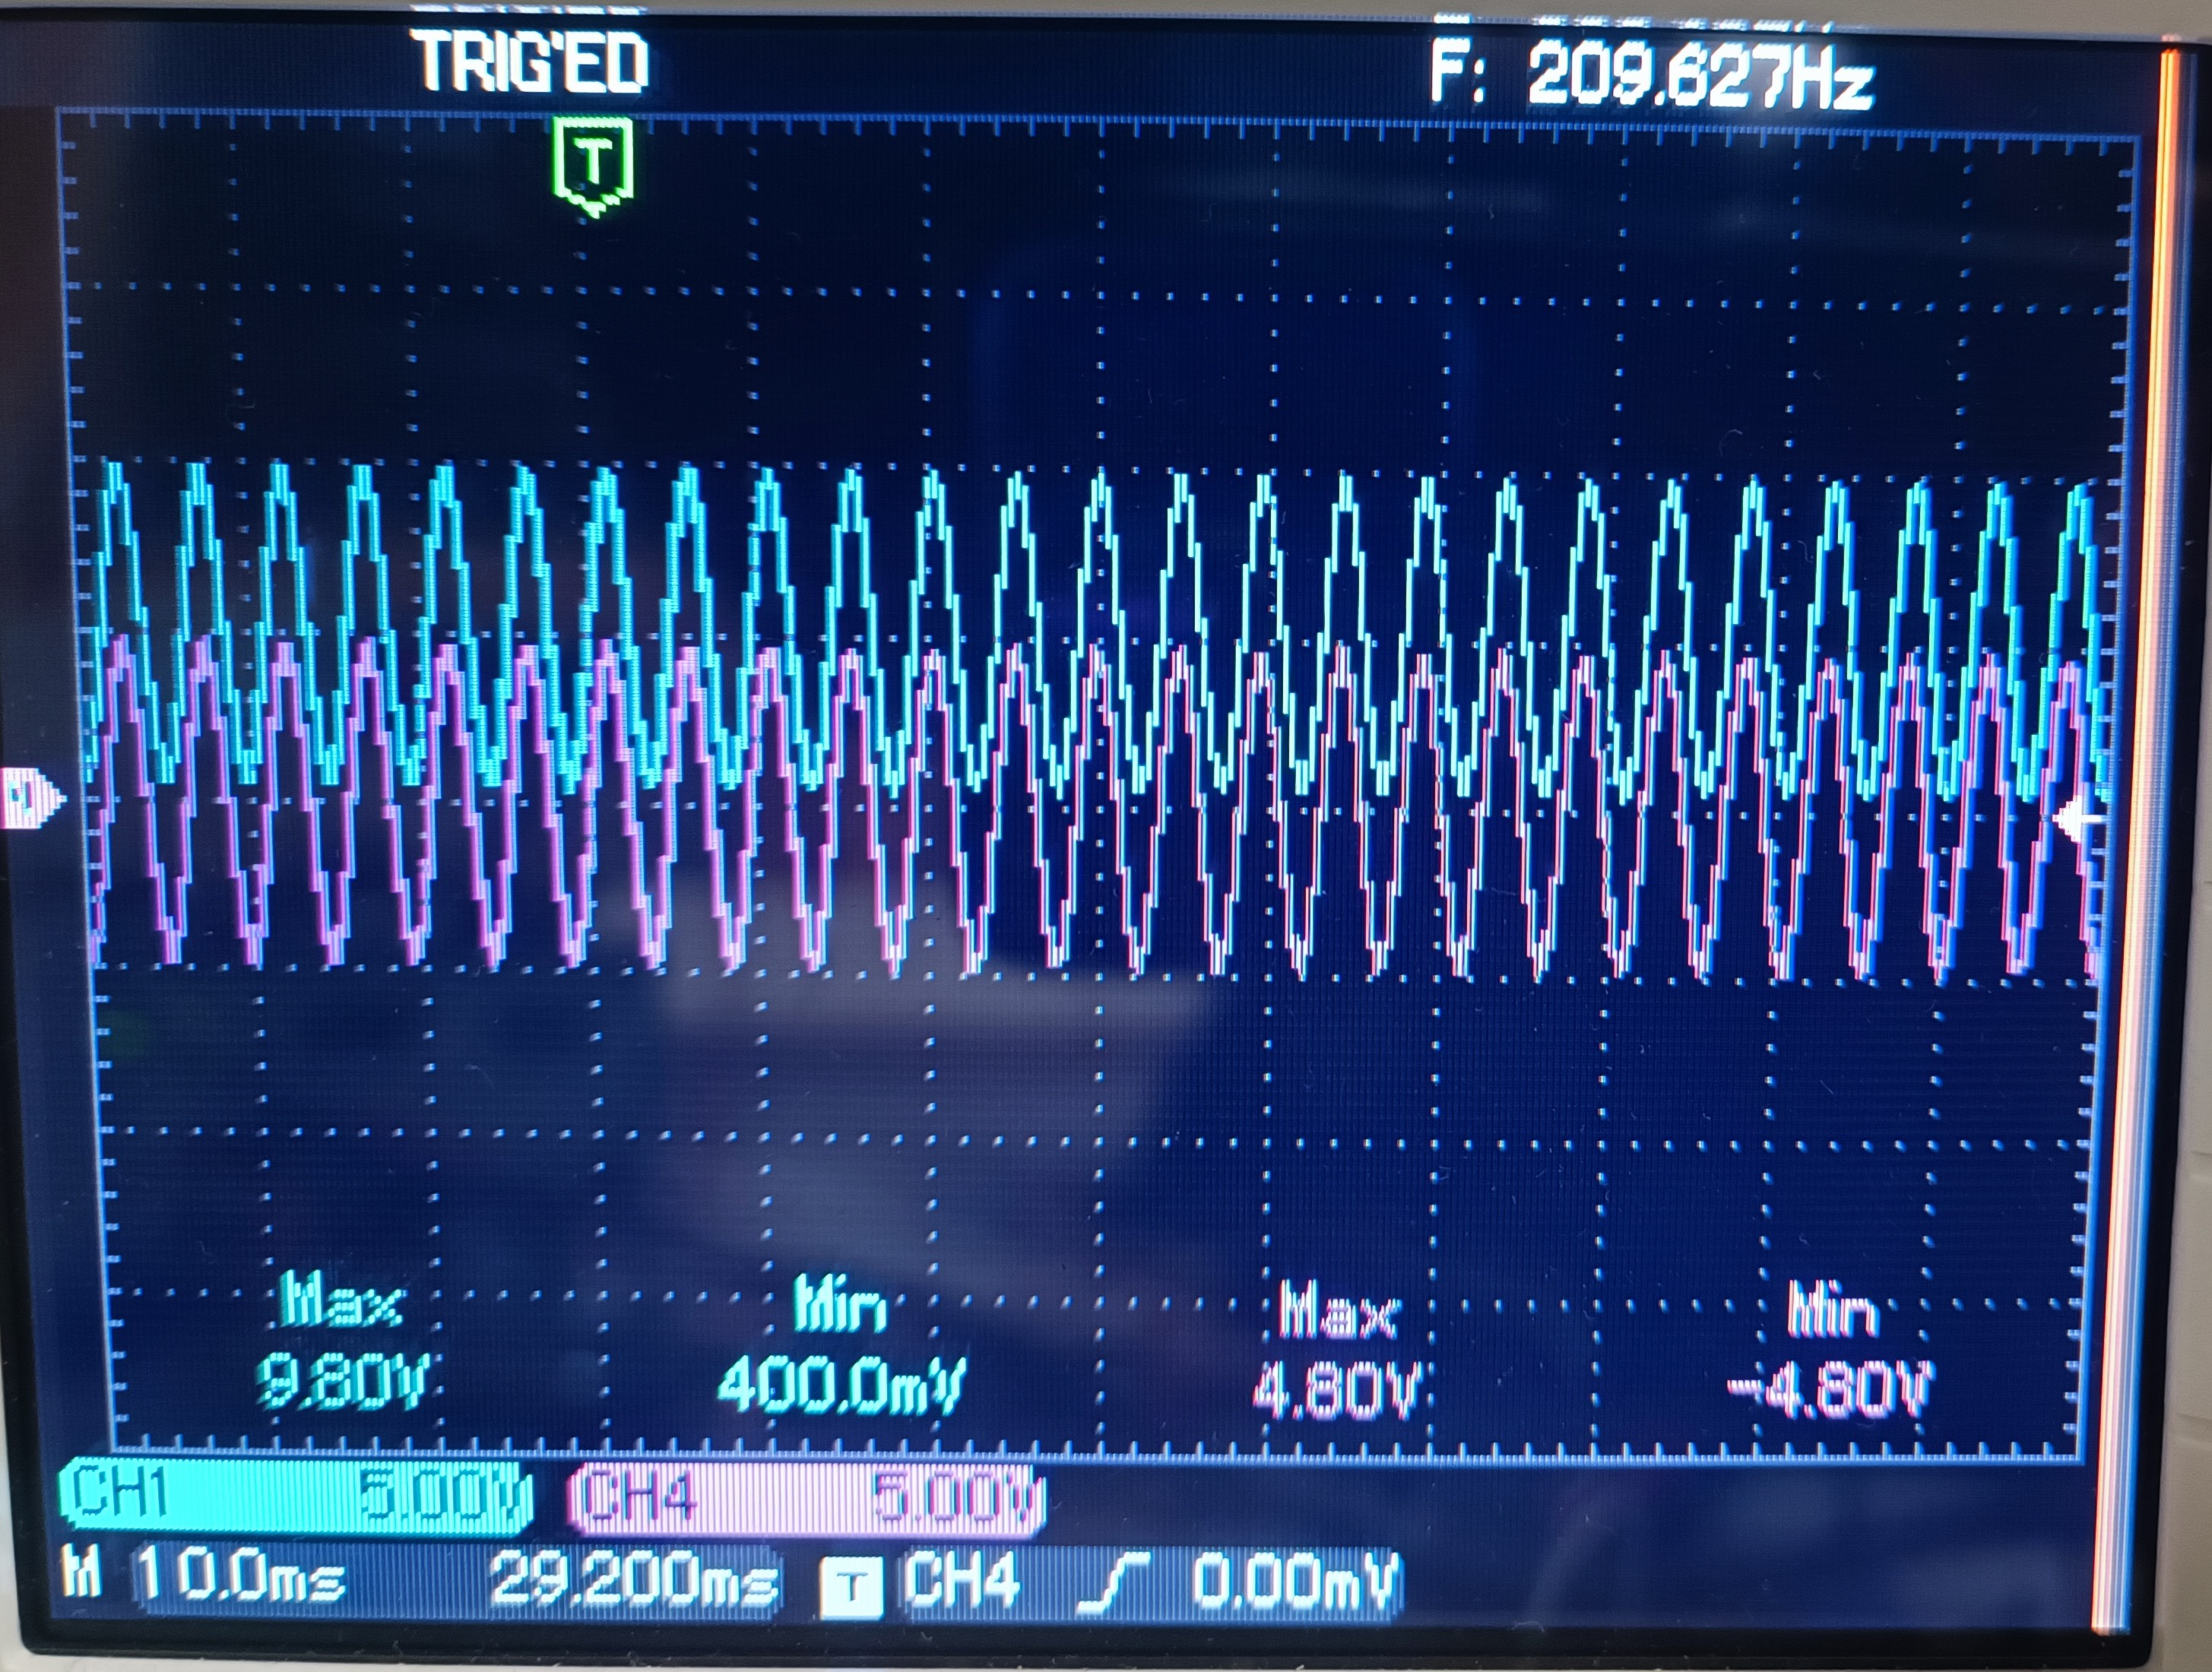
\includegraphics[width=0.7\textwidth]{images/messung_adder.jpg}
%	\caption{Messung von $U_{in}$ (lila) und $U_3$ (blau)}
%\end{figure}

\subsection{Spannungsteiler}
\label{Spannungsteiler}

Zuletzt wird die Spannung $U_3$, welche aus \textit{Opamp2} gegeben wird, geteilt, sodass
sie im Bereich $[0, 3.3]V$ für den GPIO Pin liegt.
Der Spannungsteiler $(R_5, R_6)$ teilt $U_3$ dabei zu
$U_{GPIO} = U_3 \cdot \frac{R_6}{(R_5 + R_7) + R_6} = U_3 \cdot \frac{100 \Omega}{330 \Omega}$. \newline
Dadurch ergibt sich ein Spannungsbereich für $U_{GPIO}$ von
$[0, 10 \cdot \frac{100}{330}]V = [0, 3.3]V$.
\begin{figure}[h!]
	\centering
	\includegraphics[scale=0.7]{images/schematic\_teil3\_spannungsteiler.png}
	\caption{Spannungsteiler zu $U_{GPIO}$, Ausschnitt aus \ref{Gesamte_Schematic}}
\end{figure}
\newline
Die bereinigte Spannung $U_{GPIO}$ wird nun an den GPIO Pin des Mikrocontrollers angeschlossen.



